%_______________________________________________________________________________________________________________________________%
%*******************************************************************************************************************************%
%===============================================================================================================================%
%------------------------------------------------------ Cn-MultiFigs.tex -------------------------------------------------------%
%===============================================================================================================================%
%*******************************************************************************************************************************%
% File: Cn-MultiFigs.tex
% Description: This file is used to validate float formatting & \caption behavior WHEN(N>= 10 figures) relative to the 
%       behavior FOR ALL other figures w/ N<10.
% Usage: <static>
%
%
%_______________________________________________________________________________________________________________________________%
% Last Updated in December, 2023
%_______________________________________________________________________________________________________________________________%
%-------------------------------------------------------------------------------------------------------------------------------%
	\begin{figure}
	  \centering
	  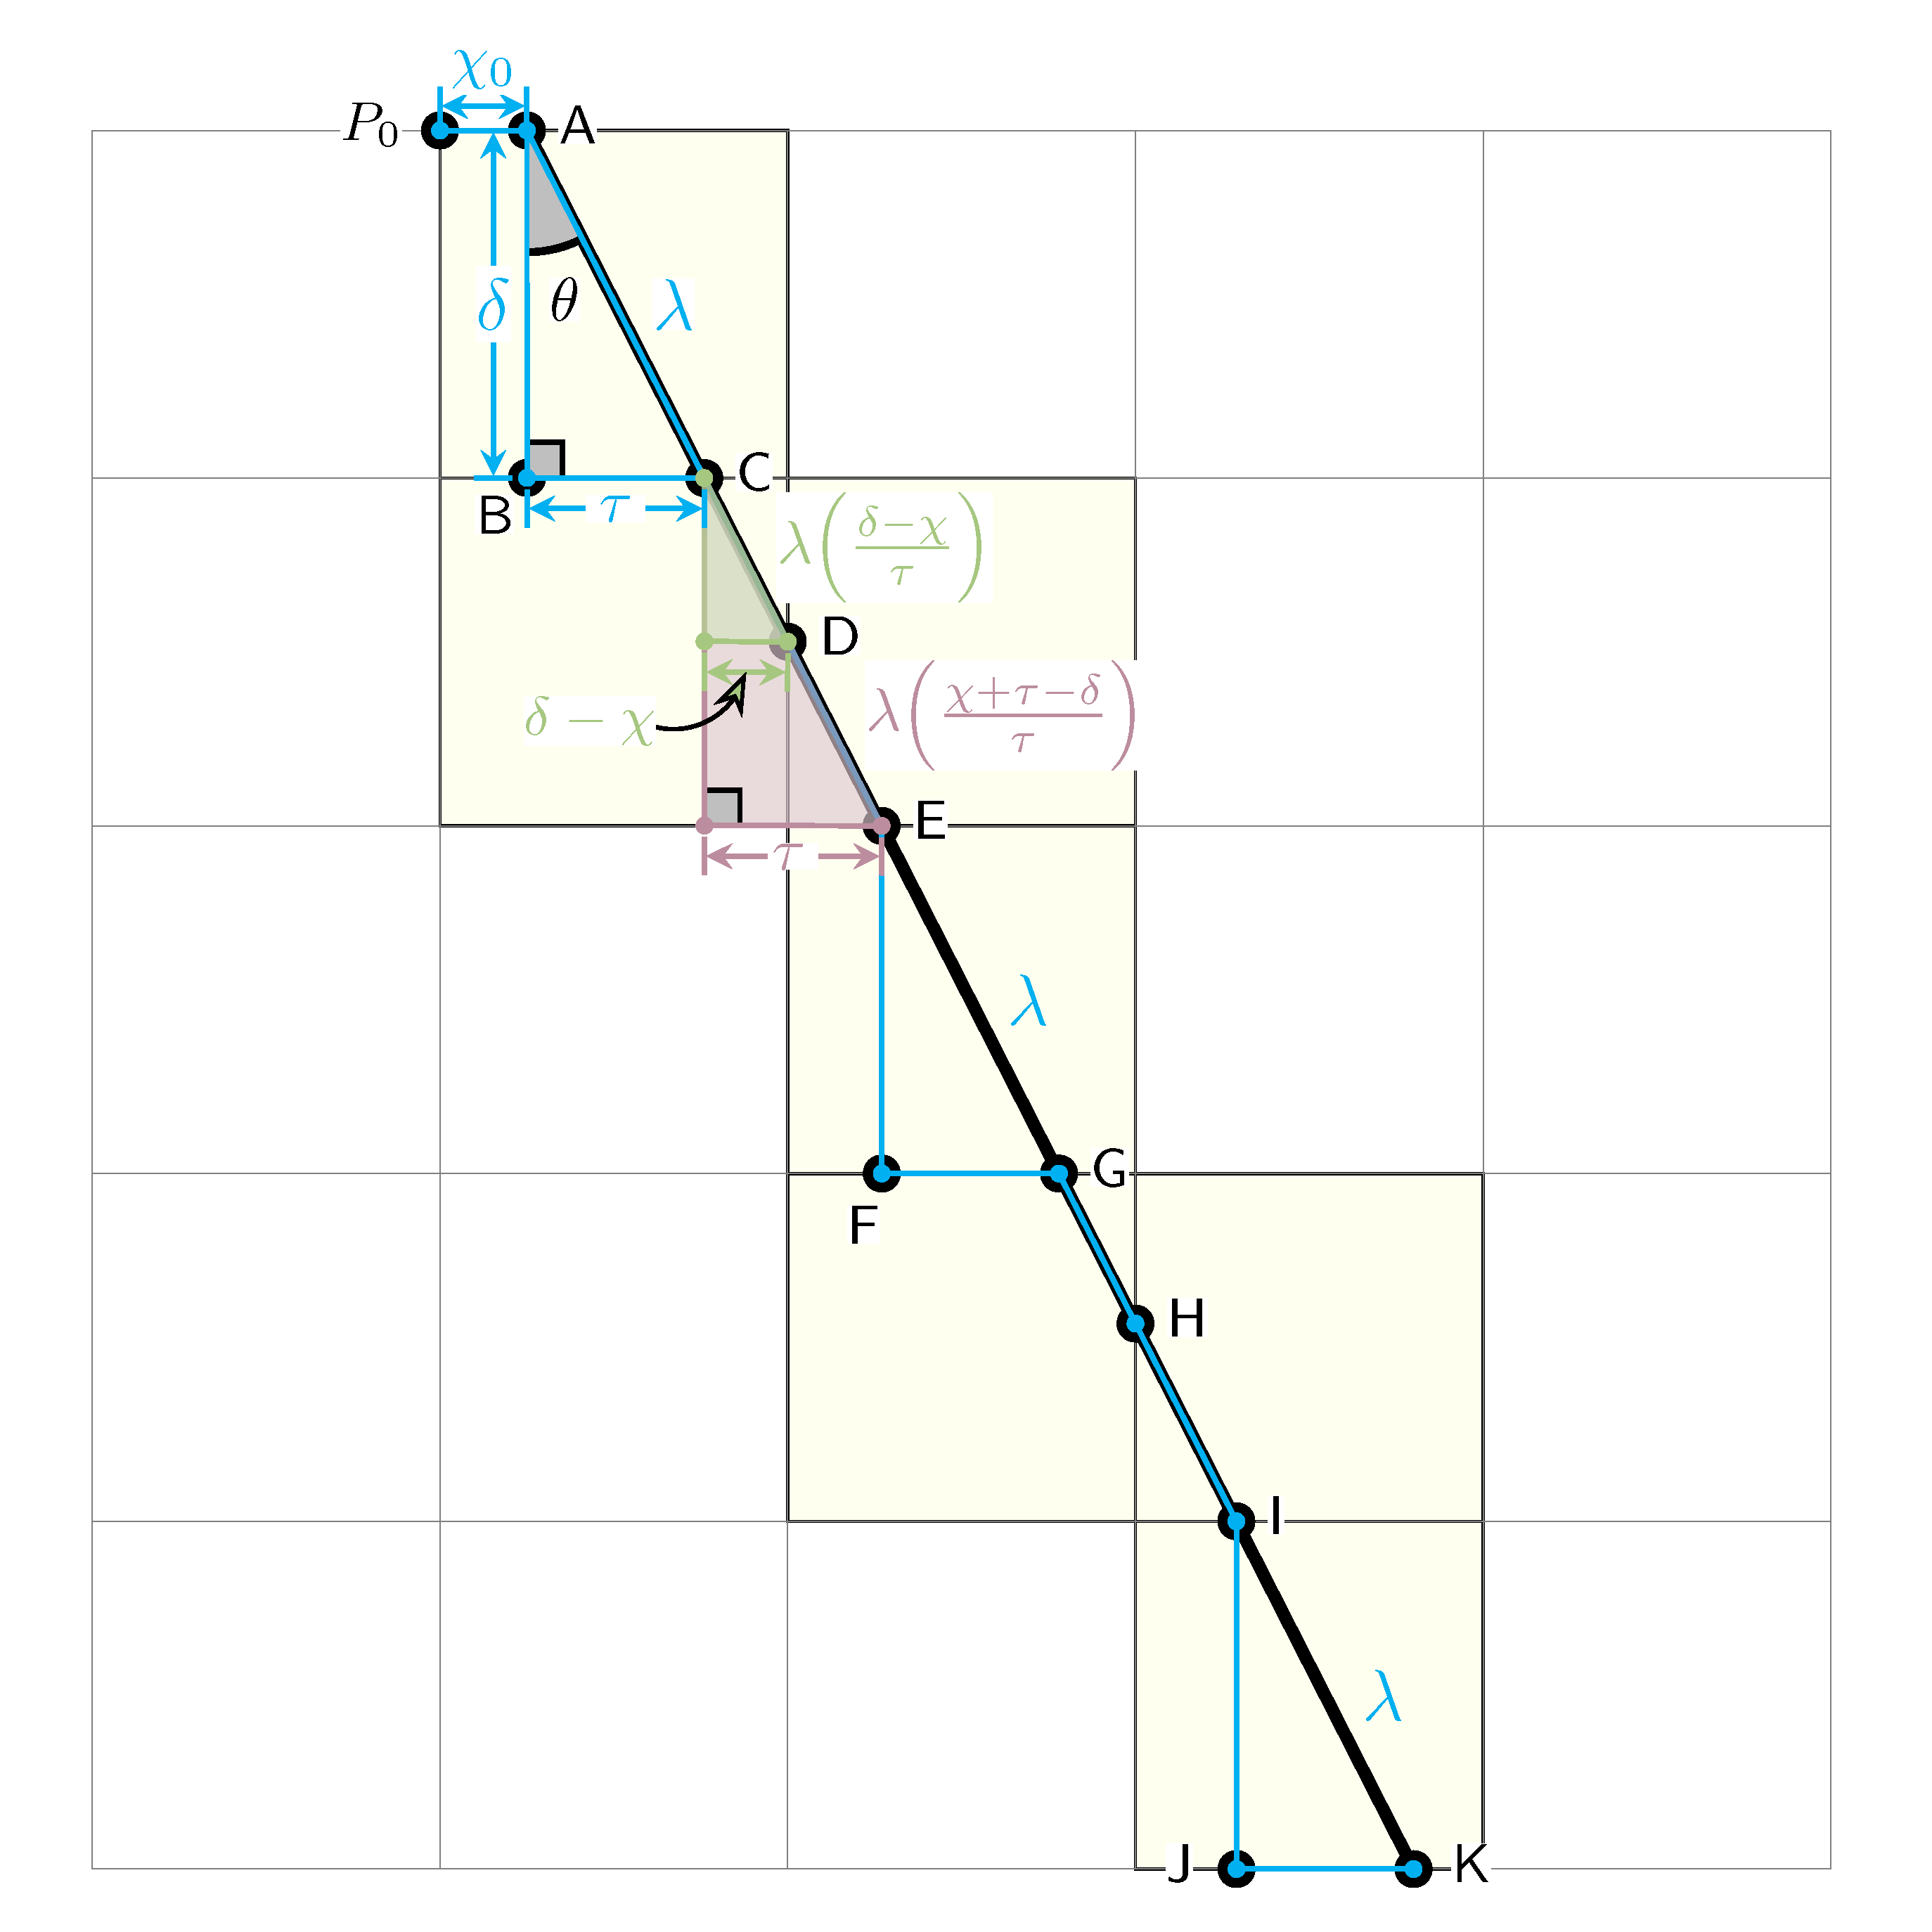
\includegraphics[width=4cm]{DDA.png}
	  \caption{Hello DDA figure caption}\label{fig:DDA-figsA}
	\end{figure}
%-------------------------------------------------------------------------------------------------------------------------------%
	\begin{figure}
	  \centering
	  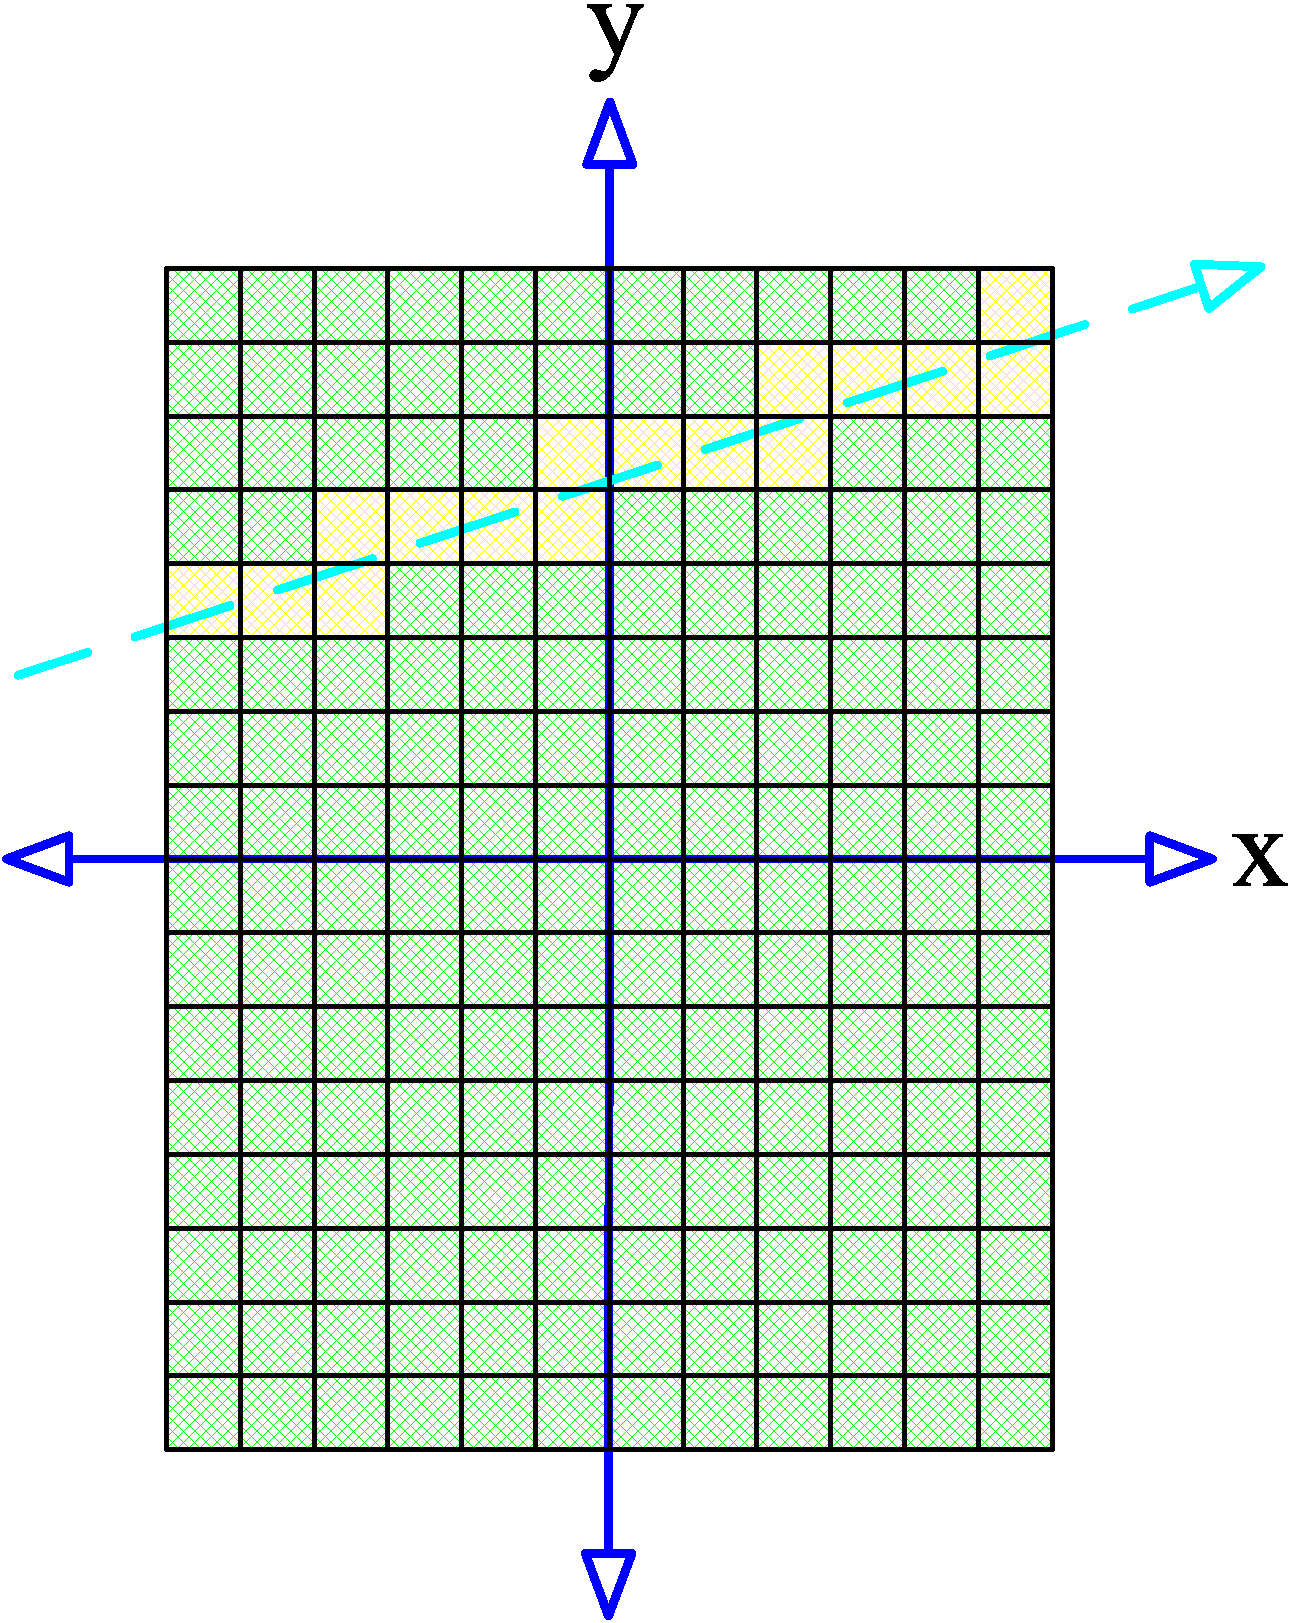
\includegraphics[width=4cm]{Space_Carving_1.png}
	  \caption{Hello DDA figure caption }\label{fig:SC-one-figsA}
	\end{figure}
%-------------------------------------------------------------------------------------------------------------------------------%
	\begin{figure}
	  \centering
	  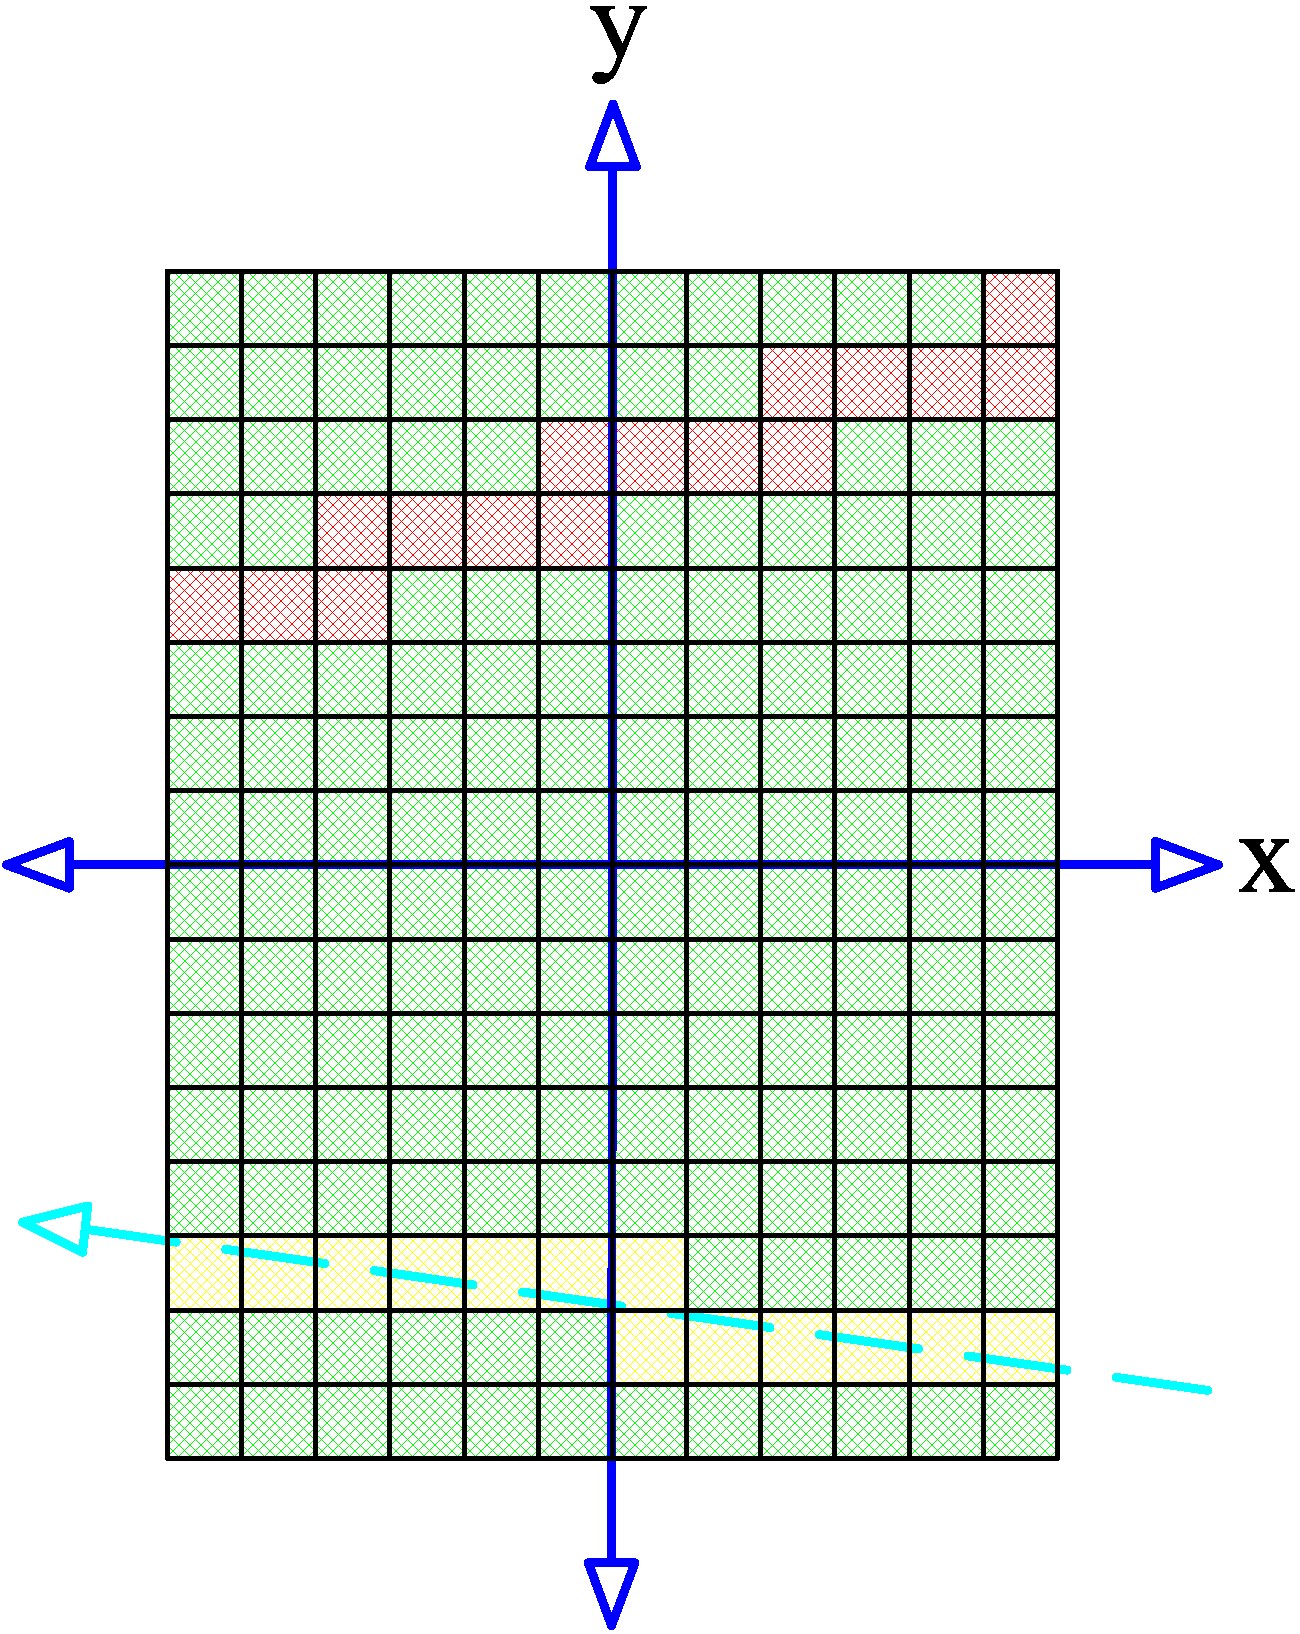
\includegraphics[width=4cm]{Space_Carving_2.png}
	  \caption{Hello DDA figure caption }\label{fig:SC-two-figsA}
	\end{figure}
%-------------------------------------------------------------------------------------------------------------------------------%
	\begin{figure}
	  \centering
	  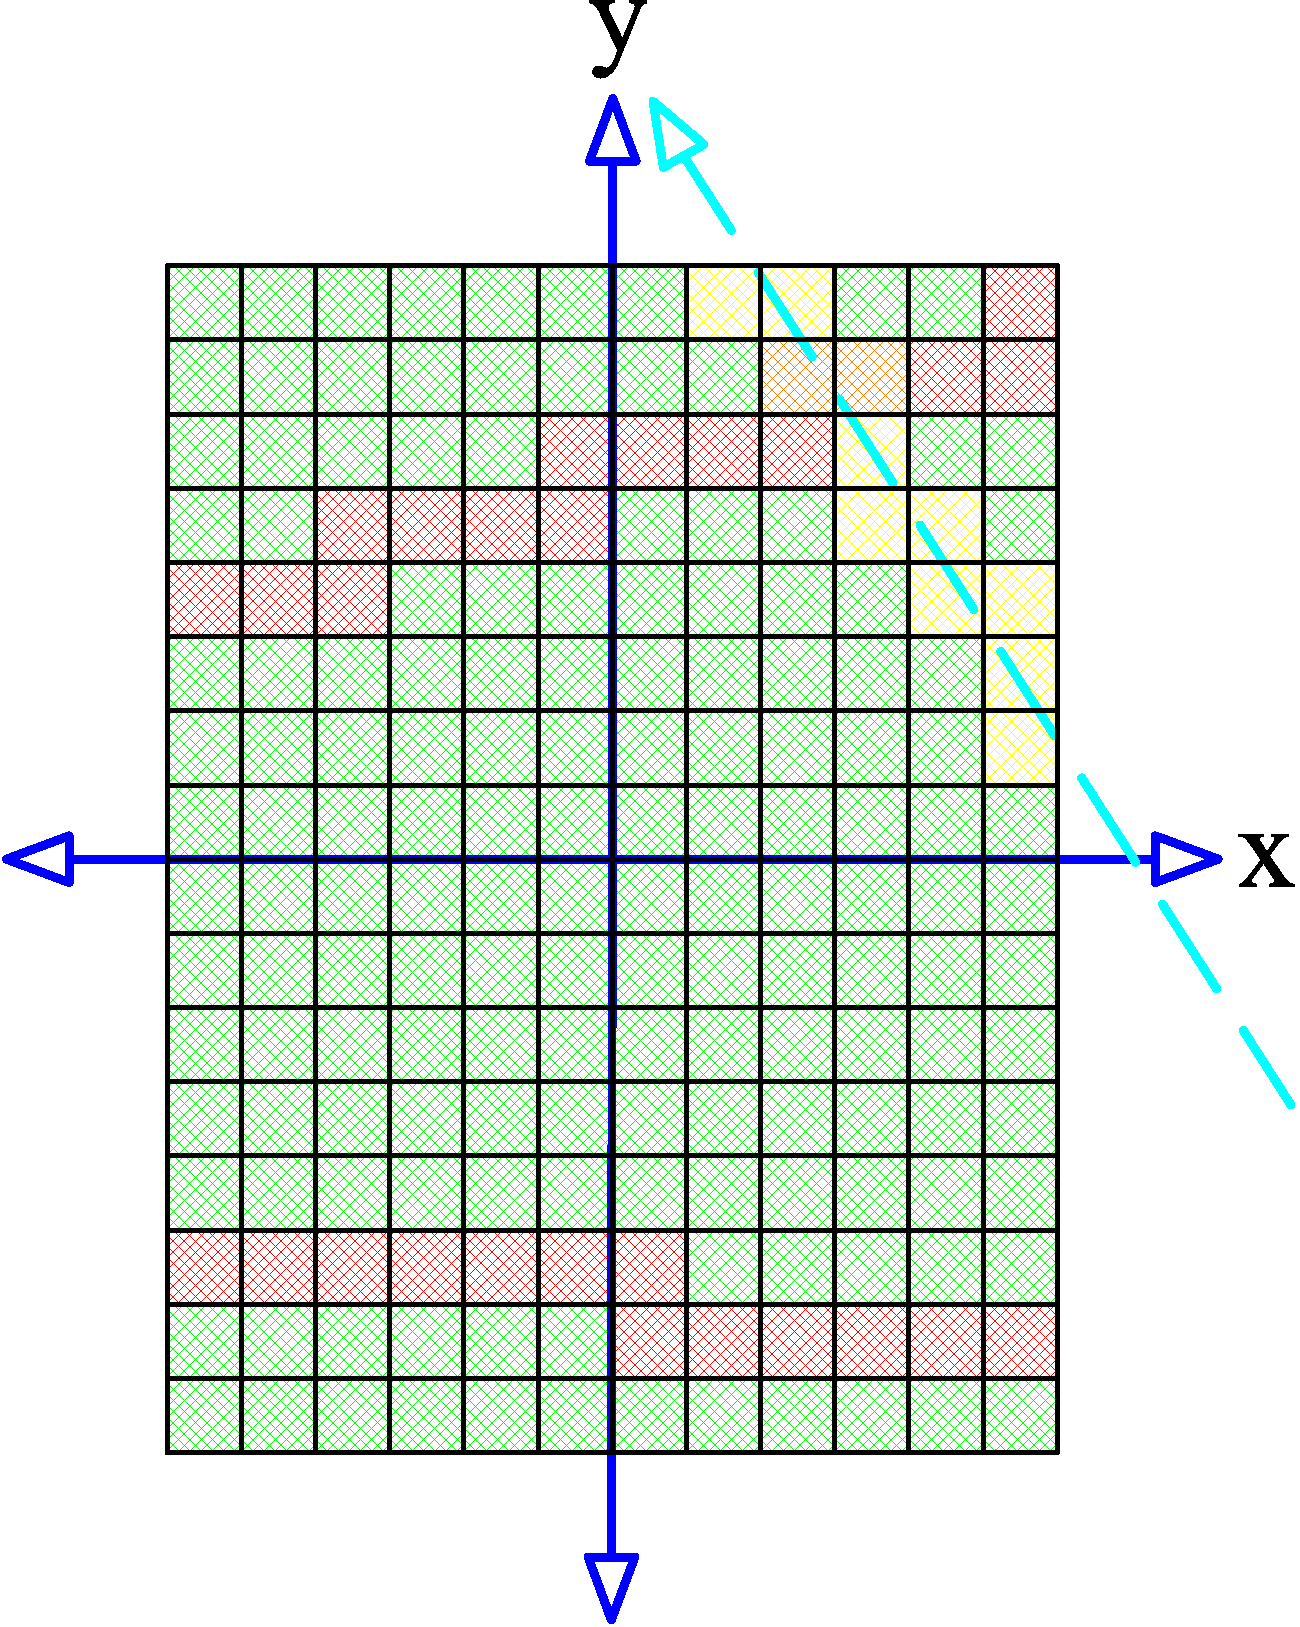
\includegraphics[width=4cm]{Space_Carving_3.png}
	  \caption{Hello DDA figure caption}\label{fig:SC-three-figsA}
	\end{figure}
%-------------------------------------------------------------------------------------------------------------------------------%
	\begin{figure}
	  \centering
	  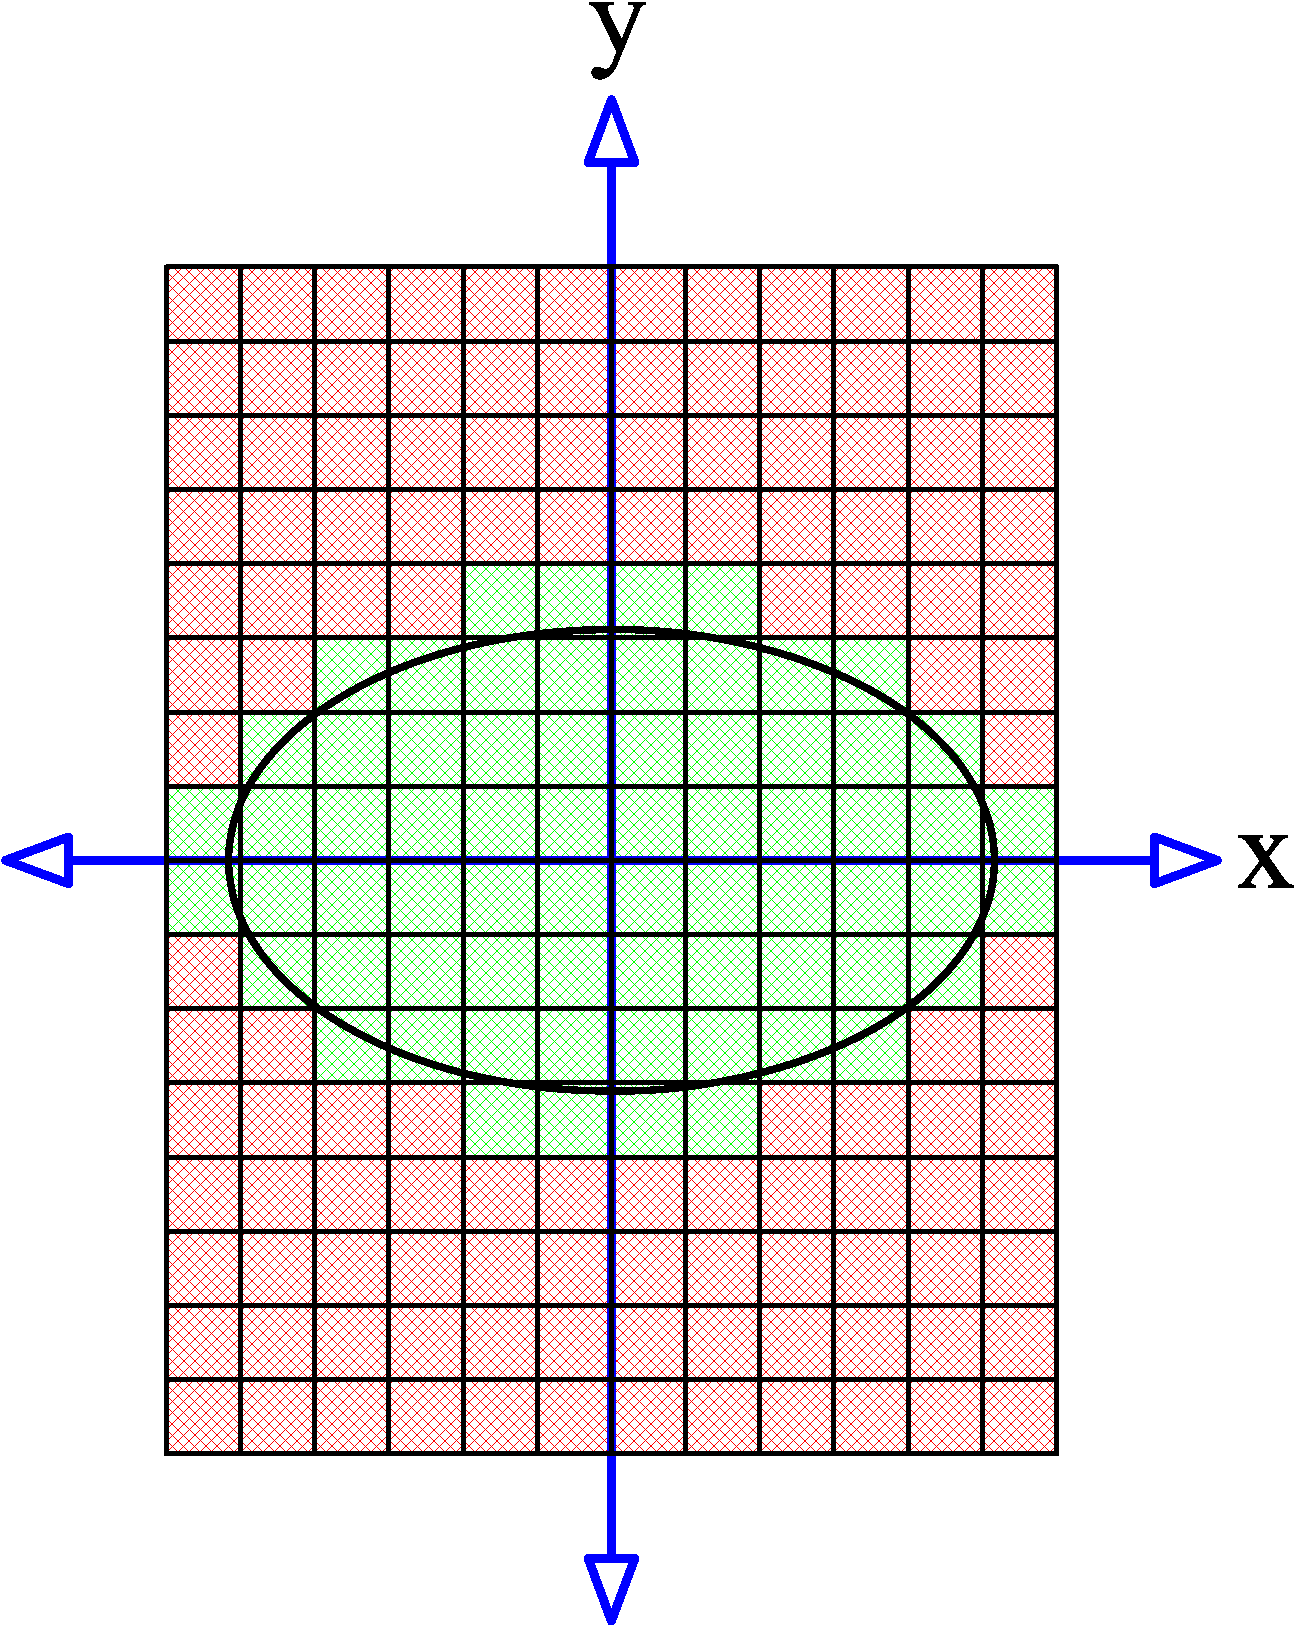
\includegraphics[width=4cm]{Space_Carving_4.png}
	  \caption{Hello DDA figure caption}\label{fig:SC-four-figsA}
	\end{figure}
%-------------------------------------------------------------------------------------------------------------------------------%
	\begin{figure}
	  \centering
	  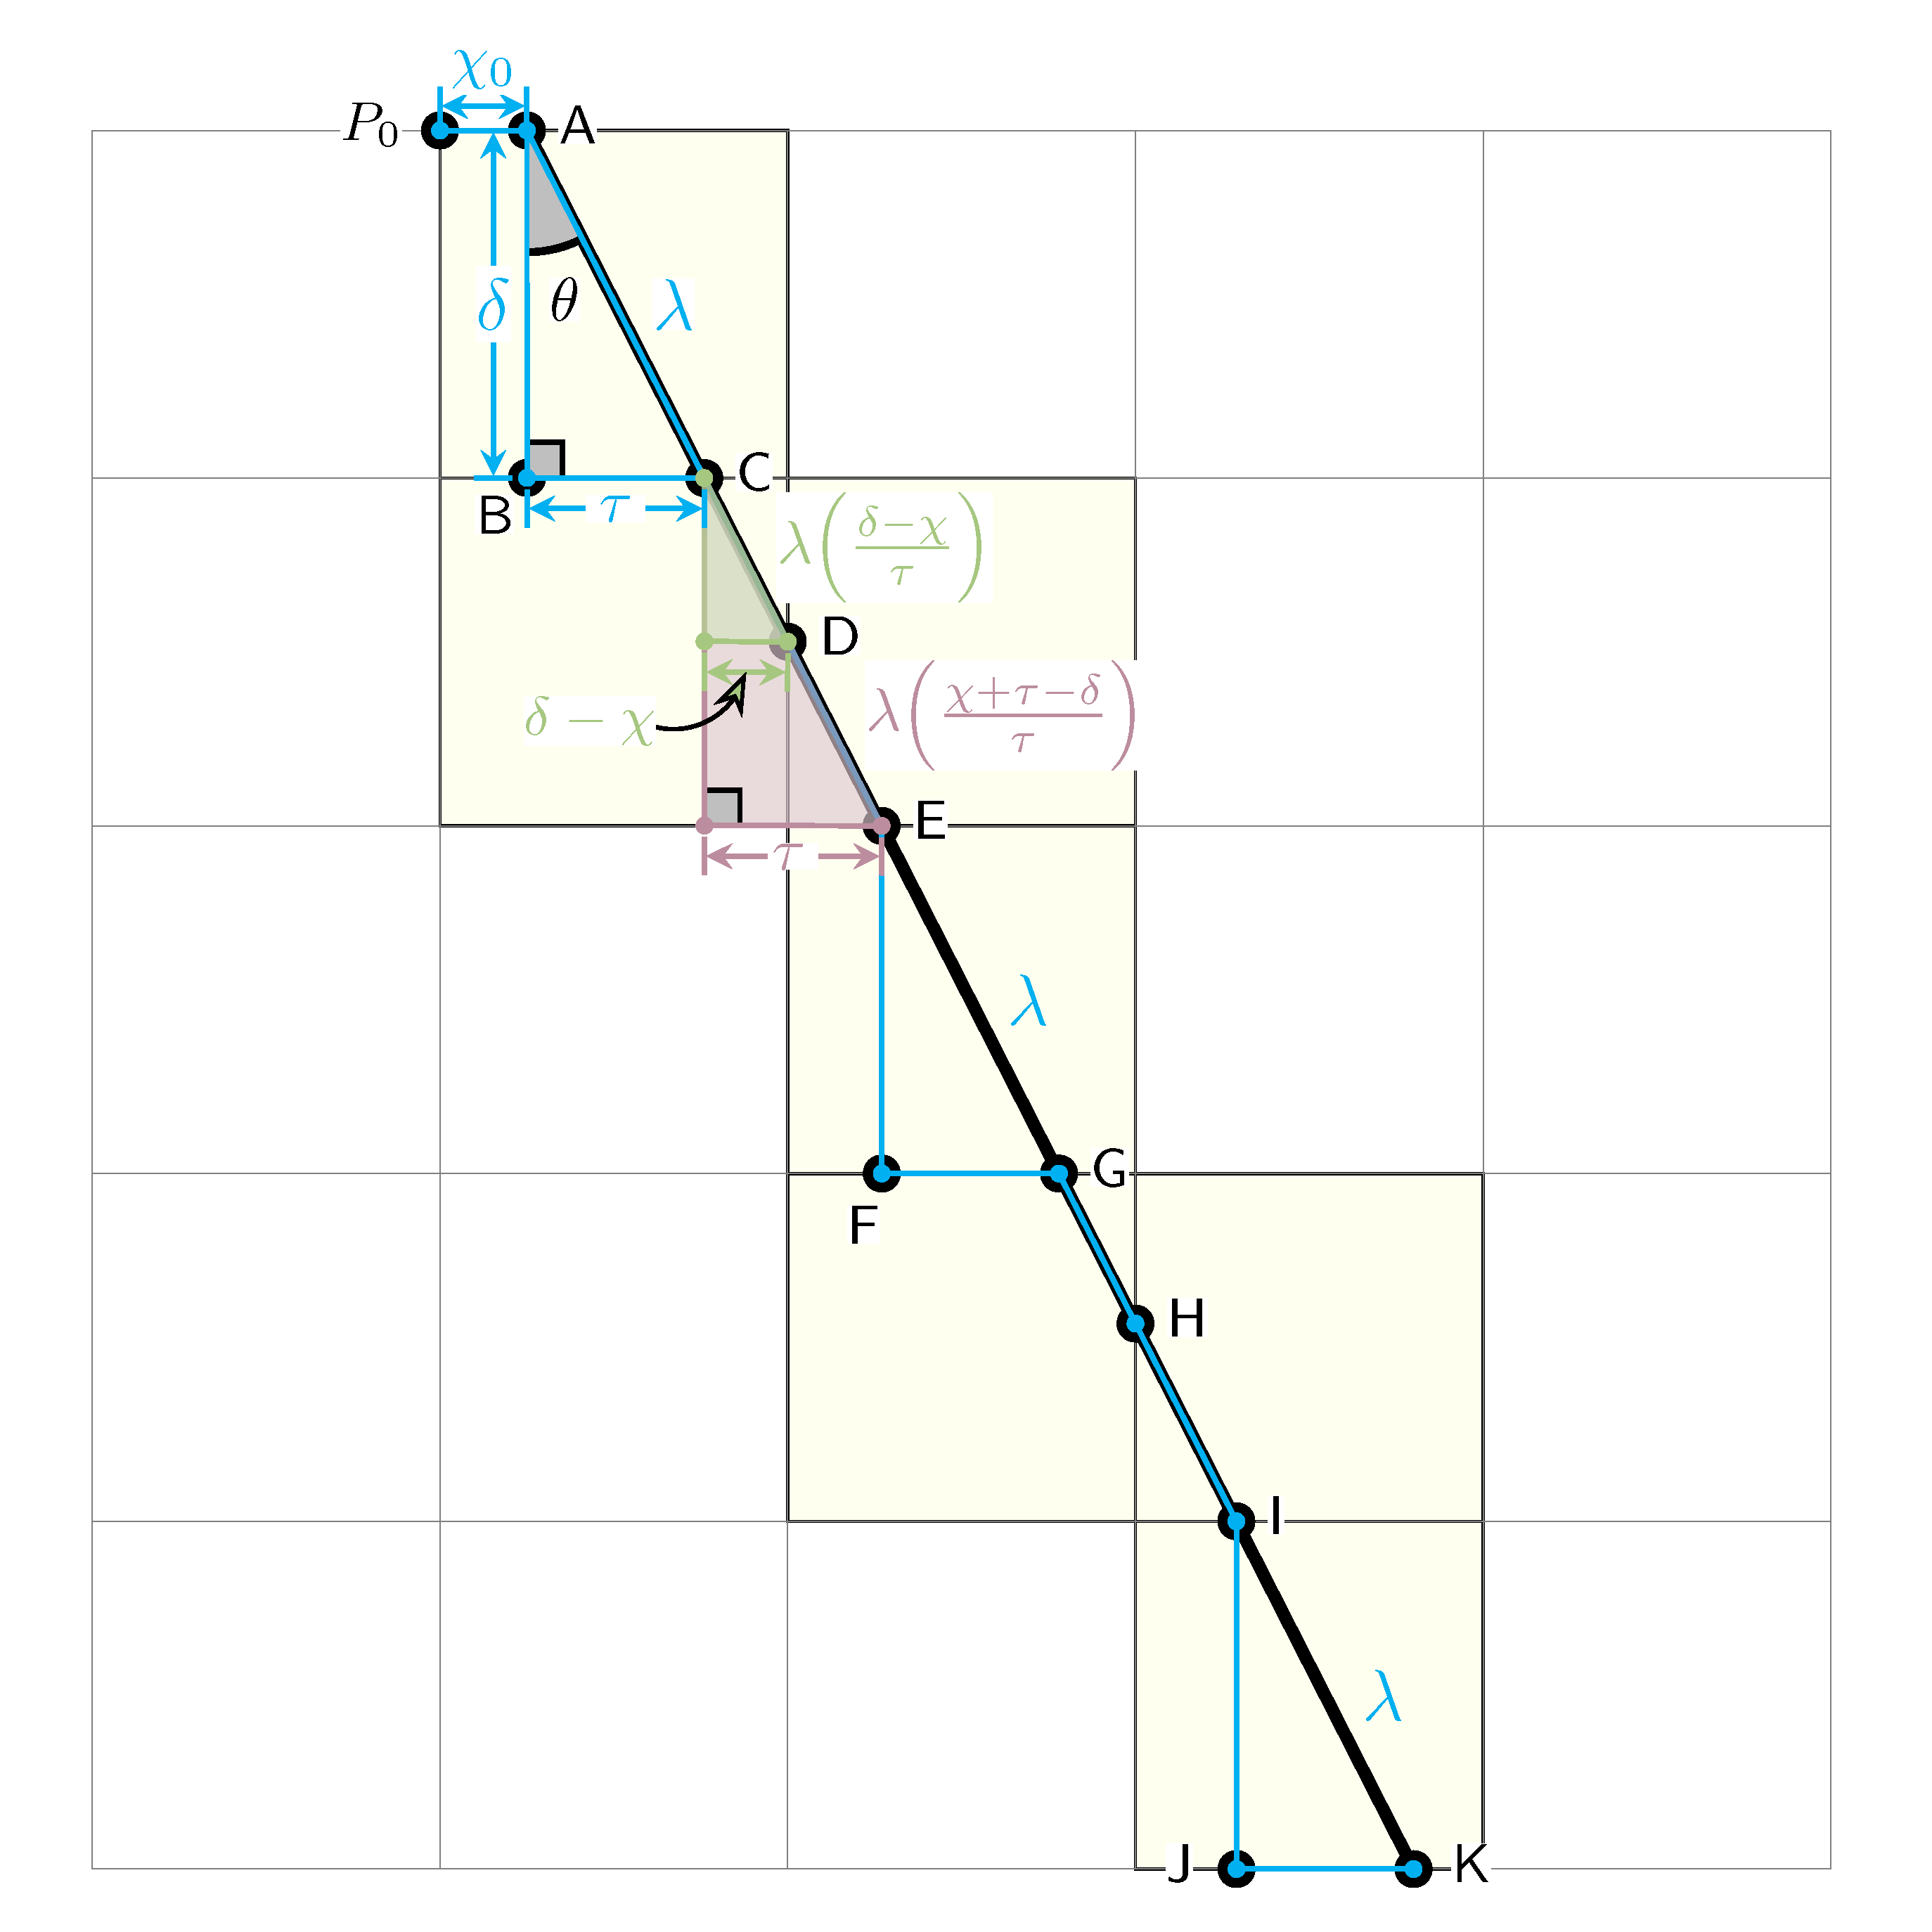
\includegraphics[width=4cm]{DDA.png}
	  \caption{Hello DDA figure caption}\label{fig:DDA-figsB}
	\end{figure}
%-------------------------------------------------------------------------------------------------------------------------------%
	\begin{figure}
	  \centering
	  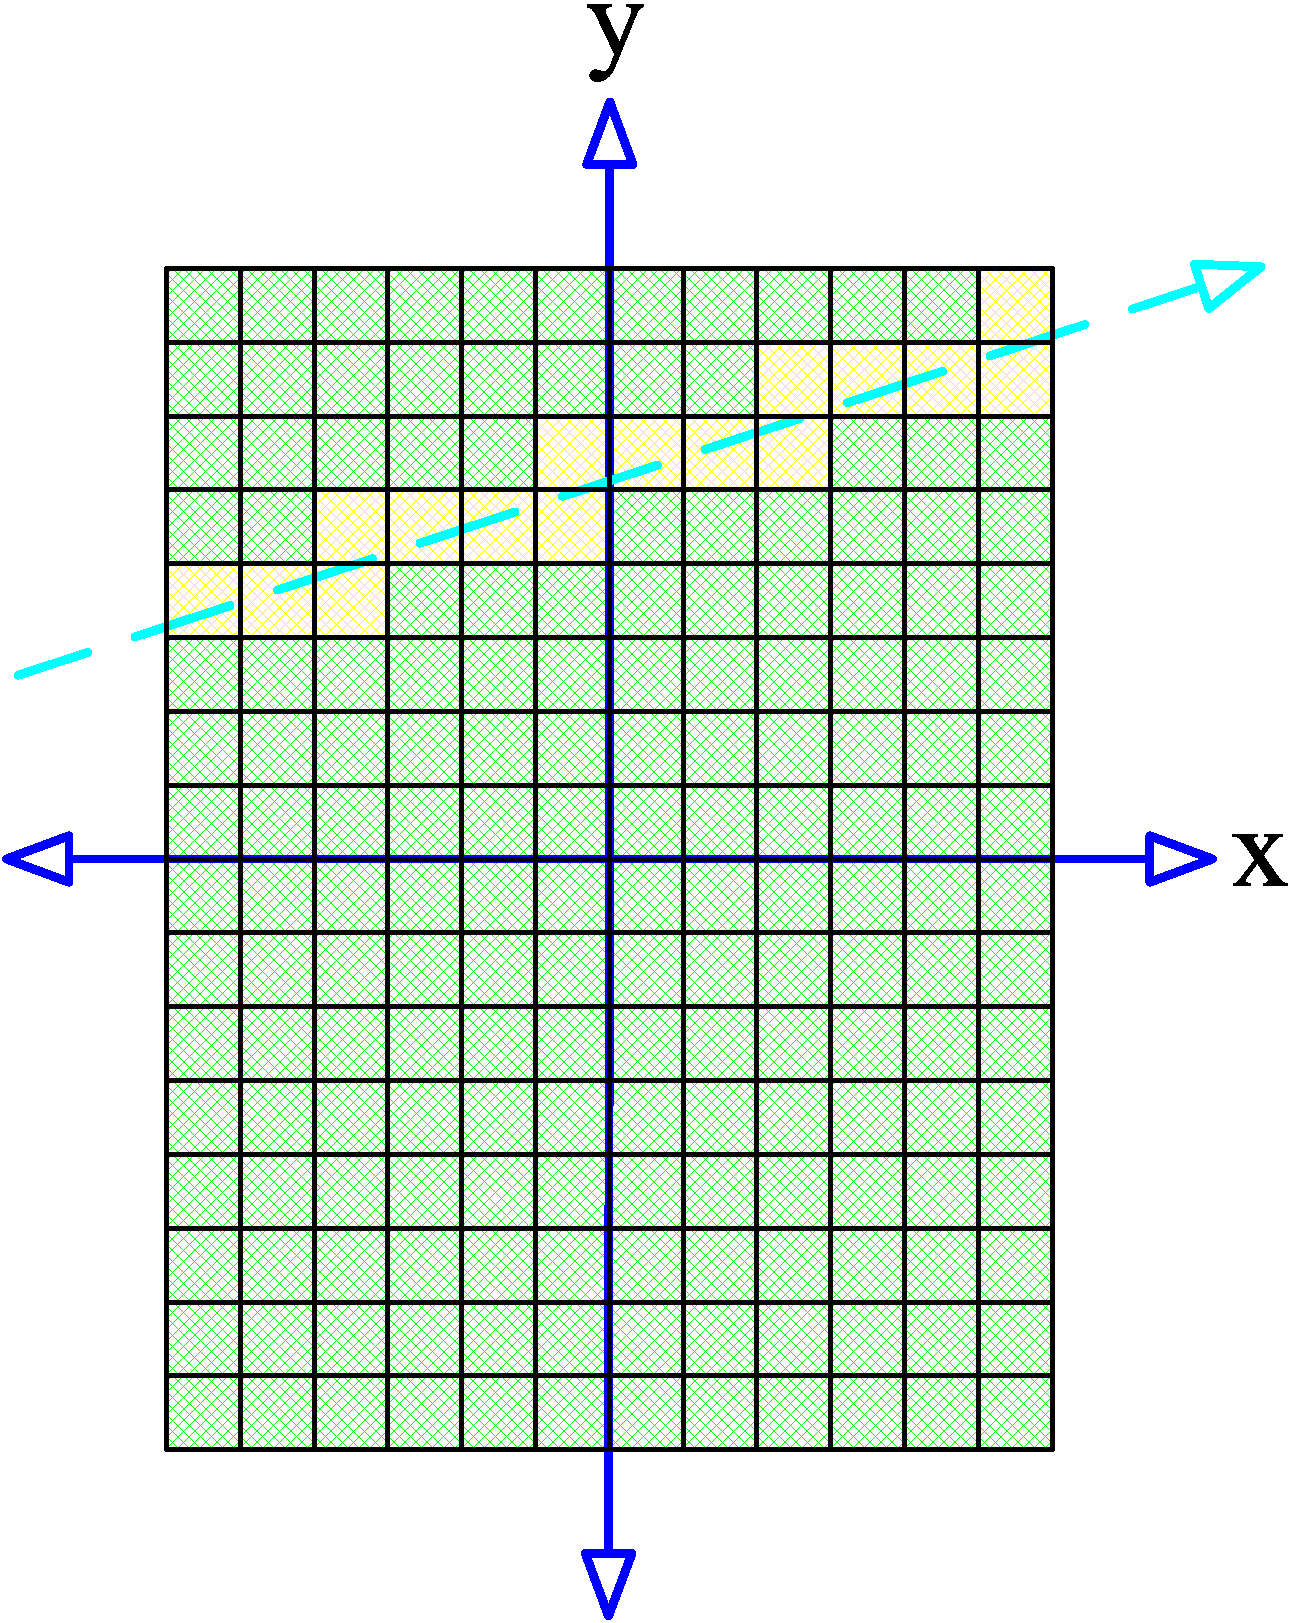
\includegraphics[width=4cm]{Space_Carving_1.png}
	  \caption{Hello DDA figure caption }\label{fig:SC-one-figsB}
	\end{figure}
%-------------------------------------------------------------------------------------------------------------------------------%
	\begin{figure}
	  \centering
	  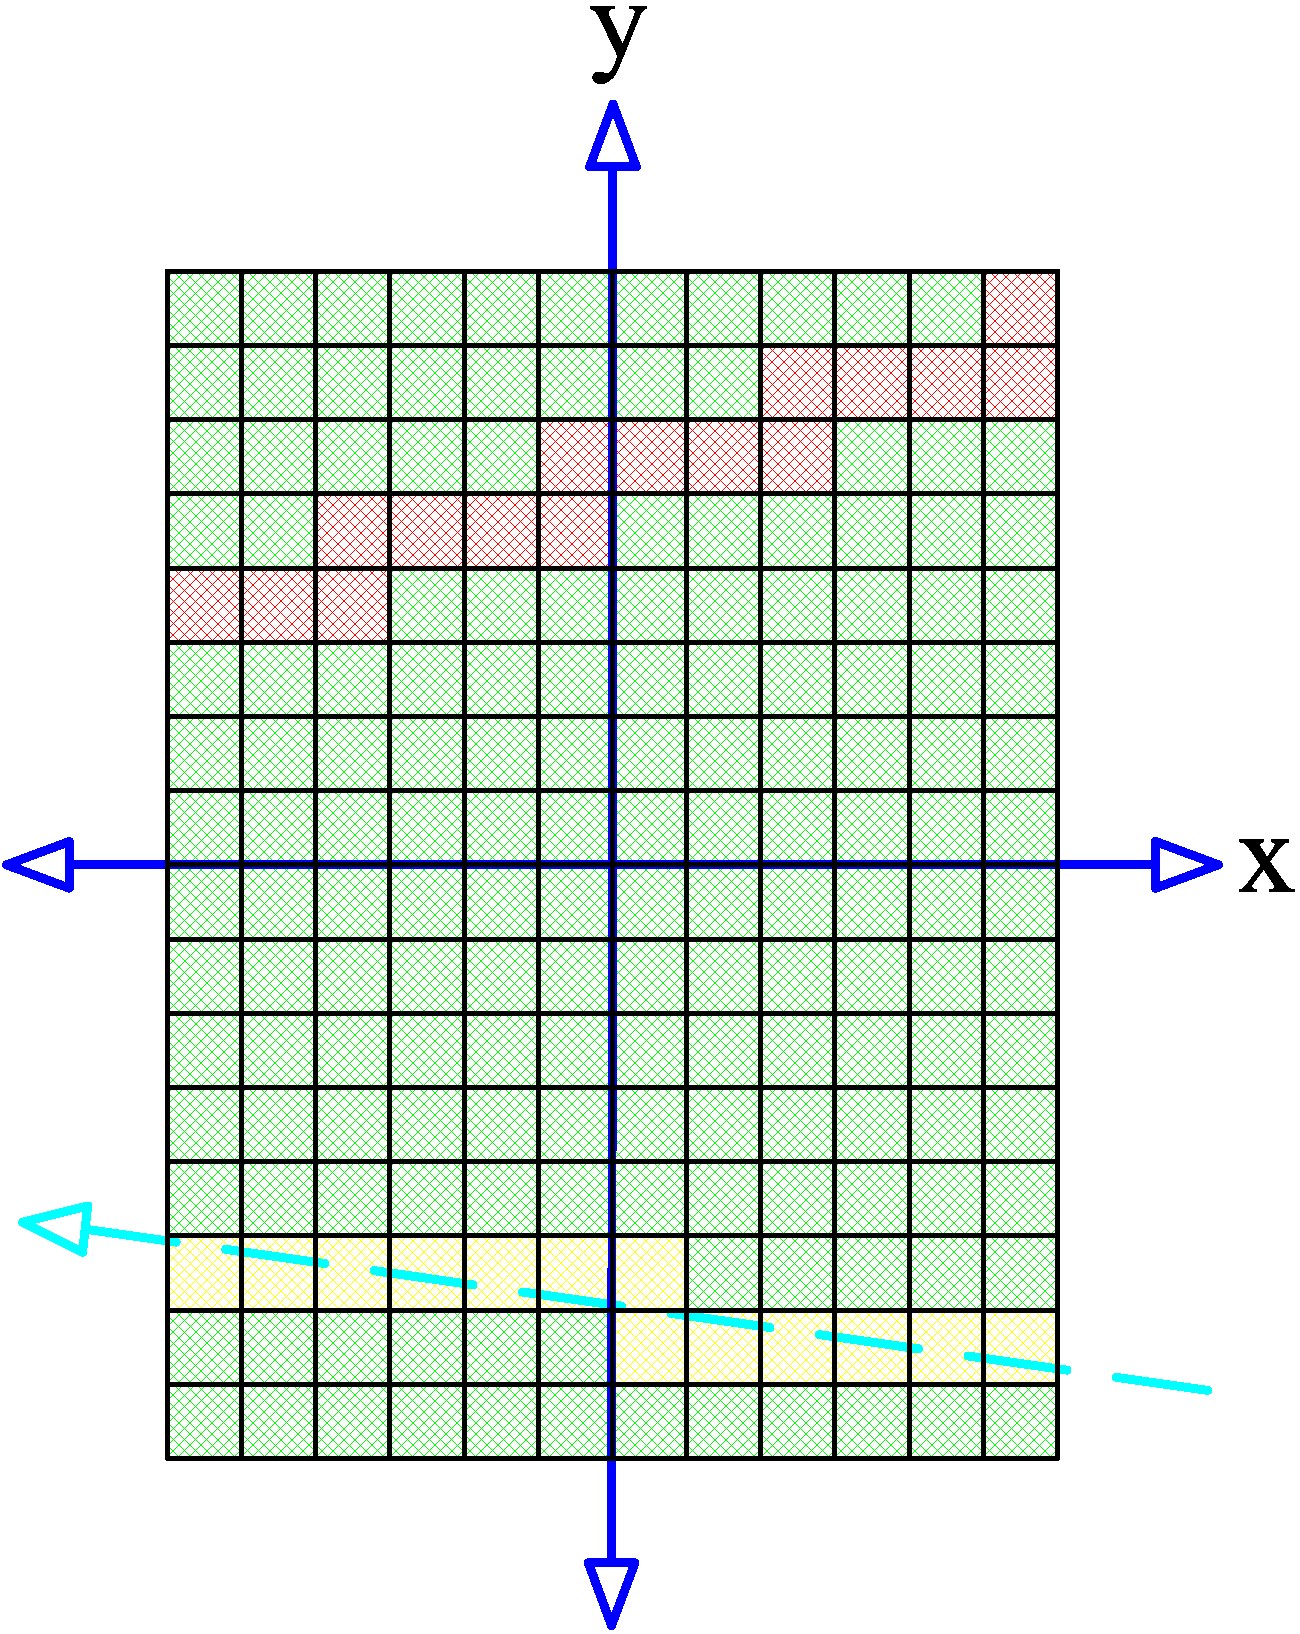
\includegraphics[width=4cm]{Space_Carving_2.png}
	  \caption{Hello DDA figure caption }\label{fig:SC-two-figsB}
	\end{figure}
%-------------------------------------------------------------------------------------------------------------------------------%
	\begin{figure}
	  \centering
	  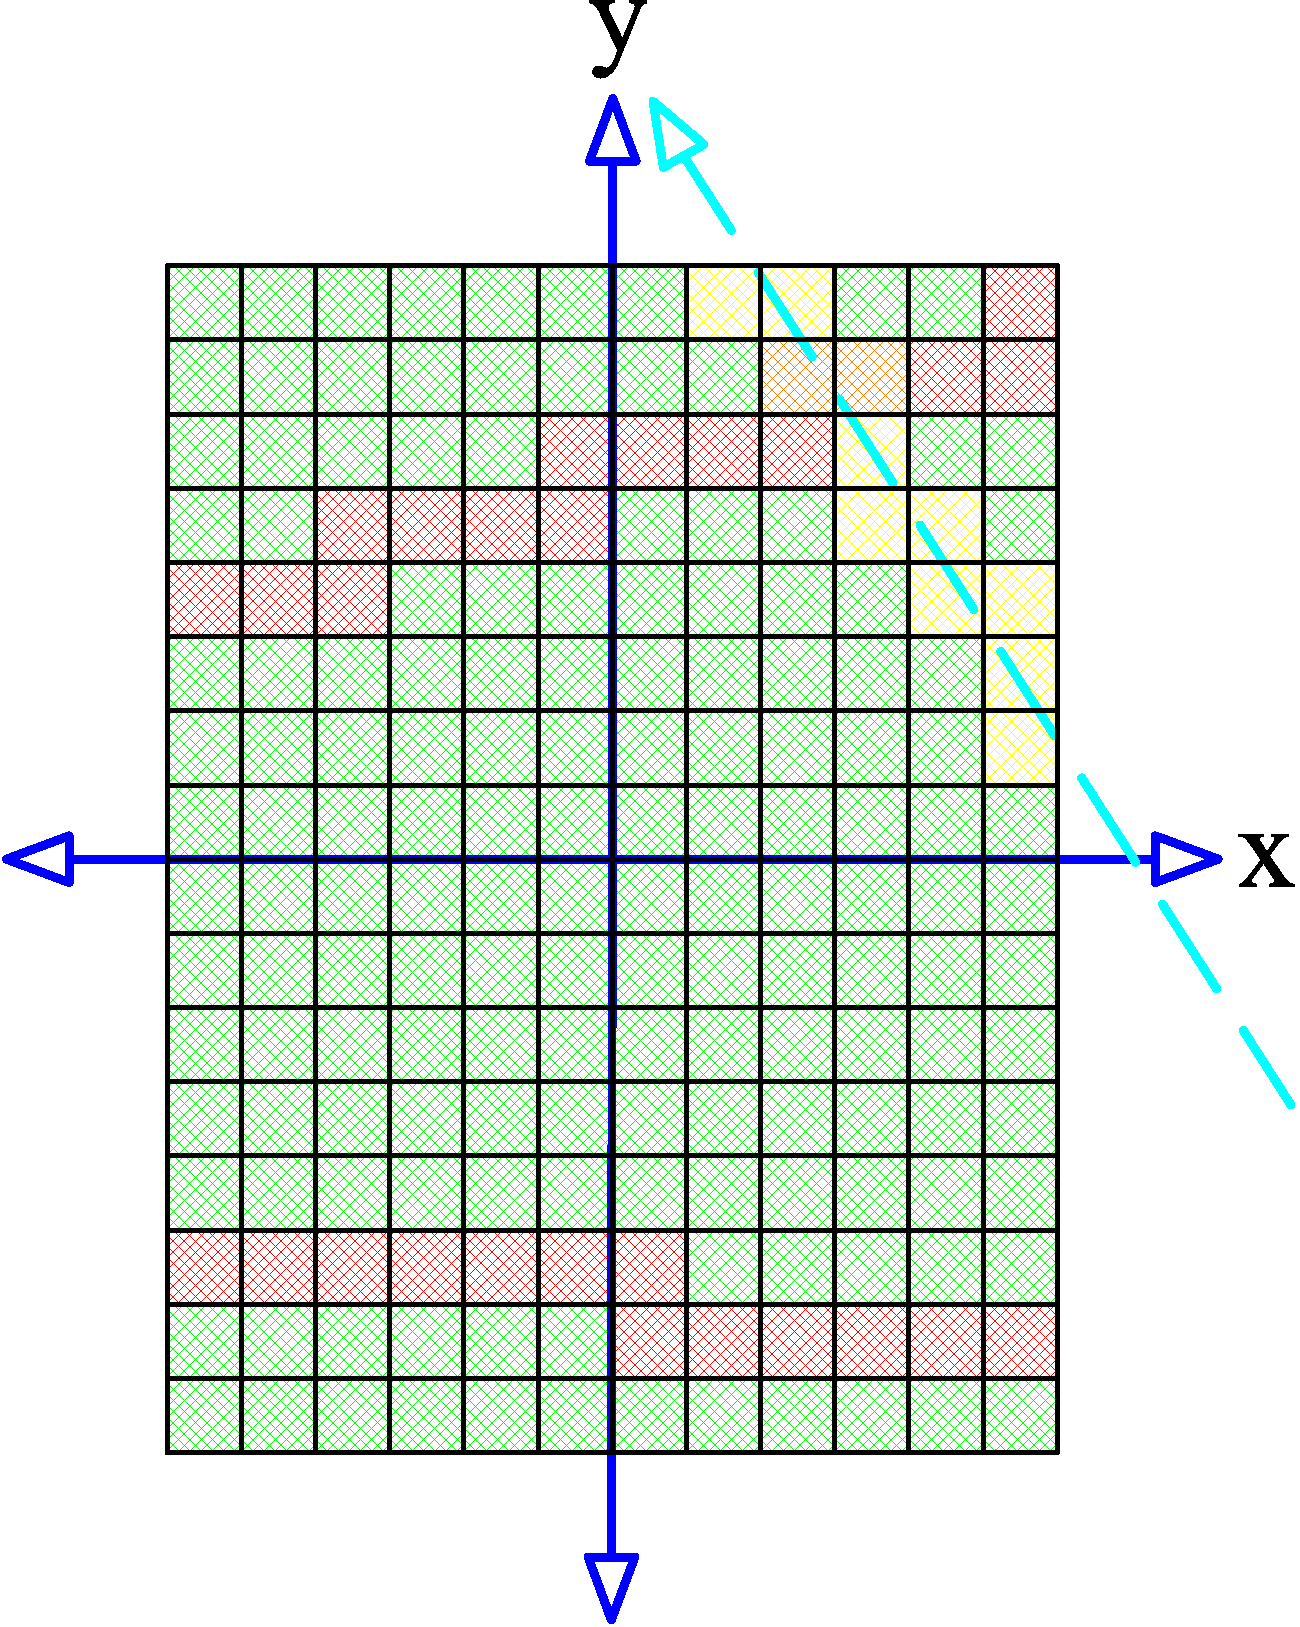
\includegraphics[width=4cm]{Space_Carving_3.png}
	  \caption{Hello DDA figure caption}\label{fig:SC-three-figsB}
	\end{figure}
%-------------------------------------------------------------------------------------------------------------------------------%
	\begin{figure}
	  \centering
	  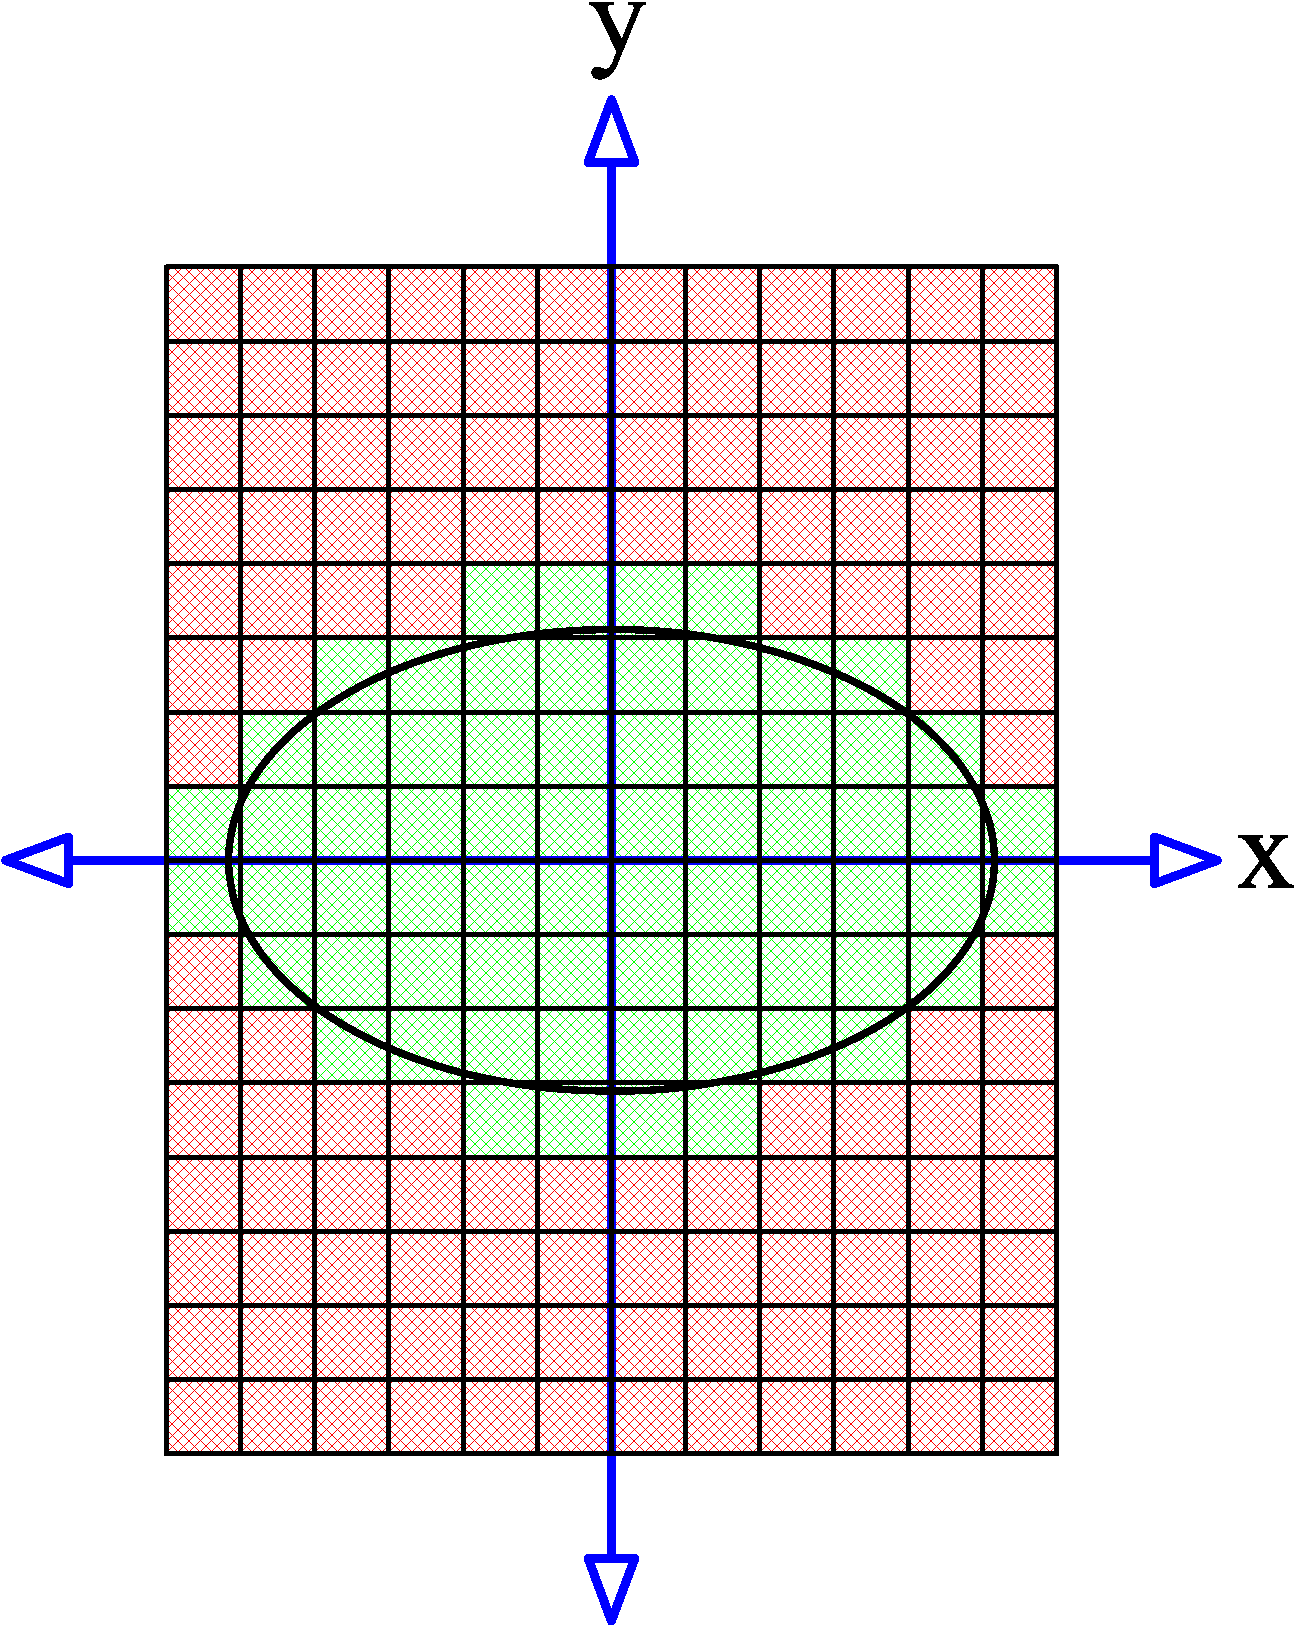
\includegraphics[width=4cm]{Space_Carving_4.png}
	  \caption{Hello DDA figure caption}\label{fig:SC-four-figsB}
	\end{figure}
%_______________________________________________________________________________________________________________________________%
%*******************************************************************************************************************************%
%===============================================================================================================================%
%---------------------------------------------------- END: Cn-MultiFigs.tex ----------------------------------------------------%
%===============================================================================================================================%
%*******************************************************************************************************************************%
\endinput 